\documentclass{beamer}
\usetheme{CambridgeUS}

\setbeamertemplate{caption}[numbered]{}

\usepackage{enumitem}
\usepackage{amsmath}
\usepackage{amssymb}
\usepackage{gensymb}
\usepackage{graphicx}
\usepackage{txfonts}

\def\inputGnumericTable{}

\usepackage[latin1]{inputenc}                                 
\usepackage{color}                                            
\usepackage{array}                                            
\usepackage{longtable}                                        
\usepackage{calc}                                             
\usepackage{multirow}                                         
\usepackage{hhline}                                           
\usepackage{ifthen}
\usepackage{caption}

\title{AI1110 \\ Assignment 6}
\author{Bandaru Naresh Kumar \\ AI21BTECH11006}
\date{}
\begin{document}
	% The title page
	\begin{frame}
		\titlepage
	\end{frame}
	
	% The table of contents
	\begin{frame}{Outline}
    		\tableofcontents
	\end{frame}
	
	% The question
	\section{Question}
	\begin{frame}{Exercise 6.40}
	The random variables x and y are of discrete type,independent with $P\{x=n\} = a_n$ , $P\{y=n\} = b_n$,n=0,1,......Show that, if $z = x+y$, then \\
	$P\{z=n\} = \sum\limits^{n}_{k=0}a_n b_{n-k}$
	\end{frame}
	
	% The solution
	\section{Solution}
	\begin{frame}{Solution}
	   \begin{figure}
	       \centering
           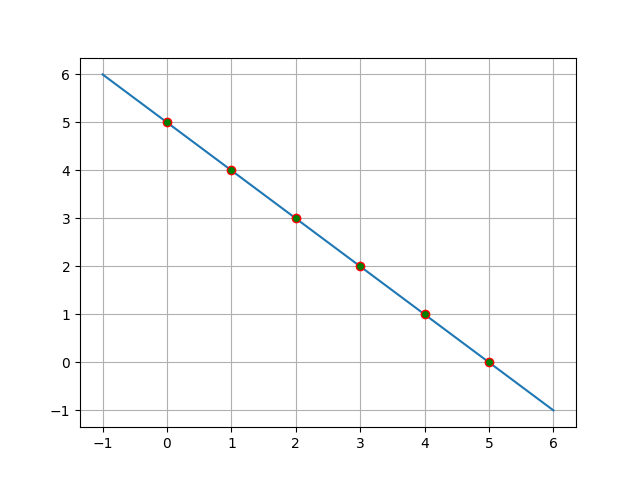
\includegraphics[scale=0.25]{figures/Figure_1.png} 
	       \caption{if n =5}
	       \label{if n=5}
	   \end{figure}
	   Since x and y are independent,
	   \begin{align}
	       P\{x=k,y=n-k\} &= P\{x=k\}P\{y=n-k\}\\
	                      &= a_n b_{n-k}
	   \end{align}
	 \end{frame}
	
	% The final answer
	\section{Answer}
	\begin{frame}{Answer}
	   Since $z=x+y$;\\
	   \begin{align}
	   \{z=n\}  &= \sum\limits^{n}_{k=0}\{x=k,y=n-k\}\\
       \implies P\{z=n\} &= \sum\limits^{n}_{k=0}P\{x=k,y=n-k\}\\
       \implies P\{z=n\} &= \sum\limits^{n}_{k=0}a_n b_{n-k}
	   \end{align}
	\end{frame}
	
\end{document}